%% Triples with equal sum and equal reciprocal sum.
%% Arithmetic companion to "How much of a hyperbolic orbifold does heat hear?".
%% Class: amsart (AMS, in TeX Live). Bibliography style: amsplain. The entries of
%% references.bib are generated from fetched records by tools/build_bib.py.
\documentclass[11pt]{amsart}

\usepackage[utf8]{inputenc}
\usepackage[T1]{fontenc}
\usepackage{amsmath,amssymb,amsthm}
\usepackage{graphicx}
\usepackage{booktabs}
\usepackage{array}
\usepackage{enumitem}
\usepackage[hidelinks]{hyperref}
\usepackage[margin=1.15in]{geometry}

\graphicspath{{../../}}% figures are addressed relative to the repository root

\newtheorem{theorem}{Theorem}[section]
\newtheorem{proposition}[theorem]{Proposition}
\newtheorem{lemma}[theorem]{Lemma}
\newtheorem{corollary}[theorem]{Corollary}
\newtheorem{conjecture}[theorem]{Conjecture}
\theoremstyle{definition}
\newtheorem{definition}[theorem]{Definition}
\theoremstyle{remark}
\newtheorem{remark}[theorem]{Remark}

\newcommand{\Q}{\mathbb{Q}}
\newcommand{\R}{\mathbb{R}}
\newcommand{\Z}{\mathbb{Z}}
\newcommand{\PP}{\mathbb{P}}
\newcommand{\N}{\mathcal{N}}
\newcommand{\Ncl}{\mathcal{N}_{\mathrm{cl}}}
\newcommand{\ciso}{c_{\mathrm{iso}}}
\newcommand{\Orb}{\mathcal{O}}

\hypersetup{pdftitle={Triples with equal sum and equal reciprocal sum},
  pdfauthor={Palaash Gang, Akshaj Agadi, Arjun Veluri, Jerry Wang, Jeremy Barreto, Aarin Chouthaiwale},
  pdfkeywords={equal sums of reciprocals, elliptic curves, rational points, counting}}

\begin{document}

\title{Triples with equal sum and equal reciprocal sum}

\author[P.~Gang]{Palaash Gang}
\address{Indus International School, Pune, India}
\email{palaash.gang@indusschoolpune.com}
\thanks{Corresponding author: Palaash Gang.}
\thanks{ORCID iDs: P.~Gang 0009-0006-7448-9488; A.~Agadi 0009-0009-1378-0556; A.~Veluri 0009-0001-5940-3272; J.~Wang 0009-0004-1814-275X; J.~Barreto 0009-0006-6894-7323; A.~Chouthaiwale 0009-0008-3878-7183.}

\author[A.~Agadi]{Akshaj Agadi}
\address{Texas A\&M University, College Station, Texas, USA}
\email{a0708@tamu.edu}

\author[A.~Veluri]{Arjun Veluri}
\address{Indus International School, Pune, India}
\email{arjun.v@indusschoolpune.com}

\author[J.~Wang]{Jerry Wang}
\address{University of California, Irvine, Irvine, California, USA}
\email{jerryiw@uci.edu}

\author[J.~Barreto]{Jeremy Barreto}
\address{Lawrence High School, Lawrenceville, New Jersey, USA}
\email{jeremy.barreto@ltps.info}

\author[A.~Chouthaiwale]{Aarin Chouthaiwale}
\address{DriveChange Learning and Resource Centre, Pune, India}
\email{aarinchouthaiwale@gmail.com}

\subjclass[2020]{Primary 11D25; Secondary 11G05, 11D45, 14J27}
\keywords{Equal sums of reciprocals, elliptic curves, rational points, Diophantine counting}

\begin{abstract}
We study unordered triples of positive integers $\{a,b,c\}$ with $1/a+1/b+1/c<1$ that share both their sum and their reciprocal sum with another such triple. The question comes from spectral geometry: these are exactly the pairs of hyperbolic triangle orbifolds that the first two heat invariants cannot tell apart. Following Bremner, Guy and Nowakowski, two such triples correspond to rational points on one curve of the cubic pencil $(x+y+z)(xy+yz+zx)=\Lambda xyz$, here for rational $\Lambda$; reciprocation is translation by a point of order two. From this we prove that the number $\N(X)$ of coincident pairs with sum at most $X$ satisfies $(\tfrac{3}{128\pi^4}+o(1))X(\log X)^2\le\N(X)\ll_\varepsilon X^{3+\varepsilon}$, and that the number of classes is at least $(\tfrac{3\log2}{2\pi^2}+o(1))X\log X$. Schinzel's method for the equal-sum, equal-product problem gives classes of every size. An exact enumeration of all $3.07\times10^9$ admissible triples with sum at most $4800$, extended to $6000$, gives the counts in both conventions. It shows a local growth exponent falling from $2.5$ to $1.58$. We conjecture $\N(X)=X^{1+o(1)}$.
\end{abstract}

\maketitle

\section{Introduction}\label{sec:intro}

For a triple $x=(a,b,c)$ of positive integers write $e_1,e_2,e_3$ for its elementary symmetric functions, so that its sum and its reciprocal sum are
\[
  S(x)=e_1=a+b+c,\qquad R(x)=\frac{e_2}{e_3}=\frac1a+\frac1b+\frac1c .
\]
We call $x$ \emph{admissible} if $R(x)<1$; then every entry is at least $2$. This note is about the coincidences
\[
  S(x)=S(x'),\qquad R(x)=R(x'),\qquad x\ne x'\ \text{as unordered triples}.
\]
The smallest is $\{(2,8,8),(3,3,12)\}$, with $S=18$ and $R=\frac34$.

\subsection{Motivation}
A closed hyperbolic $2$-orbifold with underlying sphere and three cone points of orders $a,b,c$ exists exactly when $R<1$, and it is then the rigid triangle orbifold $\Orb(a,b,c)$ of area $2\pi(1-R)$. The constant term of its heat-trace expansion is $\chi/6+\sum_i(m_i^2-1)/(12m_i)=(S+R-2)/12$ \cite[(5.7)]{dggw2008}, where $\chi=R-1$ is the orbifold Euler characteristic. So the first two heat invariants of $\Orb(a,b,c)$ determine, and are determined by, the pair $(S,R)$. Coincidences of $(S,R)$ are therefore exactly the pairs of non-isometric triangle orbifolds that two heat invariants do not distinguish. The spectral consequences, including what happens at $S=18$, are treated in the companion paper \cite{gangetal-heat}, which also proves that the smallest coincidence is isolated \cite[Theorem~6.8]{gangetal-heat}; this note does not restate that result. This note is about the arithmetic of the coincidences themselves.

\subsection{Conventions}\label{sec:conventions}
A \emph{class} at sum $S$ is a set of at least two distinct admissible triples with sum $S$ and a common $R$, maximal with this property. A class of size $k$ contains $\binom k2$ \emph{pairs}. Let $n(S)$ be the number of unordered pairs at sum exactly $S$, and put
\begin{equation}\label{eq:counts}
  \N(X)=\sum_{S\le X}n(S),\qquad \Ncl(X)=\#\{\text{classes with }S\le X\}.
\end{equation}
A class, or a pair, is \emph{primitive} if the greatest common divisor of all entries of all its members is $1$; this is Schinzel's definition \cite[p.~587]{schinzel1996}. If a class at sum $S$ is multiplied by $k$, the result lies in a class at sum $kS$, which may contain further triples; scaled copies are counted at their own sums.

\subsection{Results}
Section~\ref{sec:curves} recalls that a class is a finite set of positive rational points on one plane cubic
\[
  C_\Lambda:\ (x+y+z)(xy+yz+zx)=\Lambda\,xyz,\qquad \Lambda=SR=\frac{e_1e_2}{e_3},
\]
the curve of Bremner, Guy and Nowakowski \cite{bgn1993}. They studied it for integer $\Lambda$; coincidences need rational $\Lambda$ ($\Lambda=\frac{27}2$ for the smallest one), so we work with the whole pencil. In Beauville's classification it is the pencil of the row $\Gamma^0_0(6)$ of his table \cite[Th\'eor\`eme and Tableau, p.~658]{beauville1982}. Reciprocation $(a,b,c)\mapsto(1/a,1/b,1/c)$, under which Bremner, Guy and Nowakowski note that solutions occur in pairs \cite[p.~117]{bgn1993}, is translation by a point of order $2$ (Proposition~\ref{prop:dual}). After rescaling to a common sum, every triple that is not a geometric progression thereby has a partner (Corollary~\ref{cor:dual}). Our results are as follows.

\begin{theorem}[Lower bounds, Theorems~\ref{thm:iso} and~\ref{thm:loglog}]\label{thm:A}
As $X\to\infty$,
\[
  \N(X)\ \ge\ \Ncl(X)\ \ge\ \Big(\frac{3\log2}{2\pi^2}+o(1)\Big)X\log X,\qquad
  \N(X)\ \ge\ \Big(\frac{3}{128\pi^4}+o(1)\Big)X(\log X)^2 .
\]
\end{theorem}

\begin{theorem}[Classes of every size, Theorem~\ref{thm:largefibres}]\label{thm:B}
For every $k$ there are infinitely many primitive classes of size at least $k$.
\end{theorem}

The proof of Theorem~\ref{thm:B} is Schinzel's argument for triples with equal sum and equal product \cite[p.~588]{schinzel1996}, applied to $C_{155/12}$; we claim no novelty for the method (Section~\ref{sec:fibres}).

\begin{proposition}[Upper bound, Proposition~\ref{prop:upper}]\label{prop:C}
$n(S)\ll_\varepsilon S^{2+\varepsilon}$, and hence $\N(X)\ll_\varepsilon X^{3+\varepsilon}$.
\end{proposition}

Section~\ref{sec:growth} reports an exact enumeration of all admissible triples with $S\le4800$, extended to $S\le6000$, in both counting conventions. The local exponent $d\log\N/d\log X$ falls from $2.5$ near $X=100$ to $1.58$ near $X=6000$. The upper and lower bounds above are far apart, and the data cannot locate the exponent. We nevertheless make the following conjecture and explain what it would require (Section~\ref{sec:heuristic}).

\begin{conjecture}\label{conj:intro}
$\N(X)=X^{1+o(1)}$.
\end{conjecture}

\subsection{Relation to the literature}
The problem is the reciprocal-sum analogue of Guy's problem D16, triples with the same sum and the same product. Schinzel solved that problem through infinitely many positive rational points on the cubic $x_1+x_2+x_3=x_1x_2x_3=6$ \cite{schinzel1996}. Classes of every size for equal sums and equal products had been obtained earlier by Kelly \cite{kelly1989}, and Zhang and Cai extended Schinzel's theorem to $n$-tuples \cite{zhangcai2013}. Schinzel's curve is the fibre over $36$ of the invariant $(x+y+z)^3/xyz$ studied by Bremner and Guy \cite{bremnerguy1997}, just as $C_\Lambda$ is the fibre over $\Lambda$ of $e_1e_2/e_3$. On the equal-sum, equal-product curves, Sadek and El-Sissi determined the torsion: isosceles triples give points of order $6$, and triples with distinct entries give points of infinite order under a mild condition \cite[Prop.~2.5, Thm~2.8]{sadekelsissi2015}. Remark~\ref{rem:isosceles} is the analogue here. Parametric families of two, three and four triples with equal sum and equal product, and the elliptic curves of high rank they give, are constructed in \cite{ysv2024}. As far as we know, the counting function $\N(X)$, the bounds of Theorem~\ref{thm:A} and Proposition~\ref{prop:C}, and the enumeration are new; the geometry of Sections~\ref{sec:curves}--\ref{sec:dual} is largely in \cite{bgn1993} and \cite{beauville1982}, and we credit it there.

\section{The curves \texorpdfstring{$C_\Lambda$}{C\_Lambda}}\label{sec:curves}

\begin{proposition}[Classes are points on a cubic]\label{prop:reformulation}
Two triples with the same sum have the same $R$ if and only if they have the same $\Lambda=e_1e_2/e_3$. Conversely, let $x_1,\dots,x_k$ be pairwise non-proportional primitive triples of positive integers with a common $\Lambda$, let $s_i$ be the sum of $x_i$, and let $L=\operatorname{lcm}(s_1,\dots,s_k)$. Then the triples $(L/s_i)x_i$ lie in one primitive class at sum $L$, which may contain further triples. Any sum at which multiples of all the $x_i$ occur is a multiple $mL$ of $L$, and the triples there are admissible as soon as $mL>\Lambda$.
\end{proposition}

\begin{proof}
The first statement is immediate from $\Lambda=SR$. The rescaled triples have sum $L$ and $R=\Lambda/L$, and they are distinct because the $x_i$ are not proportional. If $d$ divides every entry of every $(L/s_i)x_i$ then, each $x_i$ being primitive, $d\mid L/s_i$ for all $i$, so every $s_i$ divides $L/d$; hence $L\mid L/d$ and $d=1$. An integer triple proportional to the primitive triple $x_i$ is $c\,x_i$ with $c\in\Z$, so a common sum $S$ for all of them forces $s_i\mid S$ for every $i$, that is $L\mid S$. Finally $R=\Lambda/(mL)<1$ when $mL>\Lambda$.
\end{proof}

So a class is a finite set of positive rational points on $C_\Lambda$, and scaling a class does not move its points. Bremner, Guy and Nowakowski observed the scale invariance for integer $\Lambda$ \cite[p.~117]{bgn1993}. By the arithmetic--harmonic mean inequality $\Lambda=e_1\cdot R\ge9$ at positive points, with equality only at $(1:1:1)$.

\begin{proposition}[The pencil]\label{prop:pencil}
Since $(x+y)(y+z)(z+x)=e_1e_2-e_3$, the curve $C_\Lambda$ is the member $t=1-\Lambda$ of the pencil
\[
  (X+Y)(Y+Z)(Z+X)+t\,XYZ=0
\]
of the row $\Gamma^0_0(6)$ of Beauville's table \cite[Th\'eor\`eme and Tableau, p.~658]{beauville1982}. Its singular members are at $\Lambda=\infty,1,0,9$, with fibres of types $I_6,I_3,I_2,I_1$. For every other $\Lambda$ the curve $C_\Lambda$ is smooth of genus one, and the maps
\[
  s=-\frac{4e_2}{z^2},\qquad \eta=\frac{4\Lambda(\Lambda-1)(x-y)}{x+y-(\Lambda-1)z},\qquad
  \frac{x+y}{z}=\frac{s(\Lambda-1)}{s-4\Lambda},
\]
together with $(x-y)/z=\eta\,\big((x+y)/z-\Lambda+1\big)/(4\Lambda(\Lambda-1))$, are mutually inverse $\Q$-birational maps between $C_\Lambda$ and the curve
\begin{equation}\label{eq:weierstrass}
  E_\Lambda:\ \eta^2=s\big(s^2+(\Lambda^2-6\Lambda-3)s+16\Lambda\big),\qquad
  \Delta=2^{12}\Lambda^2(\Lambda-1)^3(\Lambda-9),
\end{equation}
which is the model (6) of \cite[p.~118]{bgn1993} with $n=\Lambda$. For example, at $\Lambda=\frac{27}2$ the point $(1:4:4)$ maps to $(s,\eta)=(-6,45)$. With base point $O=(1:-1:0)$, the six base points of the pencil are torsion points: $(0:0:1)$ has order $2$, $(0:1:-1)$ and $(1:0:-1)$ have order $3$, and $(1:0:0)$ and $(0:1:0)$ have order $6$. Together with $O$ they form a cyclic group of order $6$.
\end{proposition}

\begin{proof}
The identity for $(x+y)(y+z)(z+x)$ gives the pencil, and comparison with the row of the table gives the identification. The maps and both compositions are verified symbolically, as is the discriminant. Because $c_4\ne0$ at $\Lambda=0,1,9$, the fibres there are of multiplicative type, with $\operatorname{ord}\Delta=2,3,1$. At $\Lambda=\infty$ the model is regular with $\operatorname{ord}_\infty\Delta=12-6=6$ and $\operatorname{ord}_\infty c_4=0$, which gives $I_6$. The orders of the base points follow from the chord-and-tangent law, computed exactly.
\end{proof}

The real picture is as follows. Bremner, Guy and Nowakowski call the bounded real component of their model the egg \cite[p.~118]{bgn1993}, and they observe that ``if $P$ is on the egg, then just the odd multiples of $P$ give positive solutions'' \cite[p.~119]{bgn1993}. They work with integer $n$. Since we need rational $\Lambda$, we give the argument.

\begin{lemma}[The egg]\label{lem:egg}
Let $\Lambda>9$ be rational. The positive real points of $C_\Lambda$ form one connected component of $C_\Lambda(\R)$, and it does not contain $O$. Consequently, if $P\in C_\Lambda(\Q)$ is positive then $nP$ is positive for every odd $n$ and not positive for every even $n$.
\end{lemma}

\begin{proof}
Let $\Delta^\circ$ be the open positive triangle in $\PP^2(\R)$. On $\Delta^\circ$ the function $e_1e_2/e_3$ is continuous and tends to $+\infty$ at the boundary. Near a point of an edge with one coordinate zero, $e_3\to0$ while $e_1e_2$ stays positive. Near the vertex $(1:0:0)$, at $(1:\epsilon:\delta)$, it is $(1+\epsilon+\delta)(\epsilon+\delta+\epsilon\delta)/(\epsilon\delta)\to\infty$, and likewise at the other vertices. So the positive locus $\{e_1e_2=\Lambda e_3\}\cap\Delta^\circ$ is compact. It is open in $C_\Lambda(\R)$, so it is a union of connected components. Since $\Delta>0$ for $\Lambda>9$, the group $C_\Lambda(\R)$ is isomorphic to $S^1\times\Z/2$ and has two components. The point $O$ is not positive, so the positive locus is the non-identity component, a coset of the identity component. Hence $nP$ lies on it exactly when $n$ is odd.
\end{proof}

\begin{remark}[Torsion]\label{rem:torsion}
For integer $n\notin\{0,1,9\}$ Bremner, Guy and Nowakowski show that ``in all cases except $n=10$, therefore, the torsion group is $\Z/6\Z$'' \cite[\S4, p.~120]{bgn1993}. For rational $\Lambda$ there is more. Since $(\Lambda^2-6\Lambda-3)^2-64\Lambda=(\Lambda-1)^3(\Lambda-9)$, the curve $E_\Lambda$ has full rational $2$-torsion exactly when $(\Lambda-1)(\Lambda-9)$ is a square in $\Q$. Then its torsion group contains $\Z/2\times\Z/6$. This happens on an infinite family that contains every curve through an isosceles point $(u:v:v)$, for which
\[
  \Lambda-1=\frac{2(u+v)^2}{uv},\qquad \Lambda-9=\frac{2(u-v)^2}{uv},
\]
and in particular $\Lambda=\frac{27}2$.
\end{remark}

\section{Reciprocation and the dual family}\label{sec:dual}

Bremner, Guy and Nowakowski note that solutions occur in reciprocal pairs \cite[p.~117]{bgn1993}. In the table of \cite[\S4, p.~120]{bgn1993} they record the reciprocal of a solution as its translate by the point $(0,0)$, and its permutations as translates of $\pm P$ by torsion points. We use the same structure in the plane model.

\begin{proposition}[Reciprocation is a $2$-torsion translation]\label{prop:dual}
Let $T_2=(0:0:1)$ and $\iota(x:y:z)=(yz:xz:xy)$. On every smooth $C_\Lambda$, with base point $O=(1:-1:0)$, we have $P+T_2=\iota(P)$ for every point $P$, and $2T_2=O$.
\end{proposition}

\begin{proof}
The line through $P=(p_0:p_1:p_2)$ and $T_2$ consists of the points $(p_0:p_1:w)$. The equation of $C_\Lambda$ restricted to it is quadratic in $w$ with root product $p_0p_1$, so the third intersection is $(p_0p_2:p_1p_2:p_0p_1)$. The line through $O$ and that point meets $C_\Lambda$ again at $(p_1p_2:p_0p_2:p_0p_1)=\iota(P)$, since the equation evaluated there equals $p_0p_1p_2$ times its value at $P$. Hence $P+T_2=\iota(P)$, and $2T_2=O$ because $\iota$ is an involution.
\end{proof}

\begin{corollary}[The dual family]\label{cor:dual}
For every triple $x=(a,b,c)$ of positive integers that is not a geometric progression,
\[
  \big\{\,e_2(x)\,(a,b,c),\ e_1(x)\,(bc,ca,ab)\,\big\},
\]
divided by the greatest common divisor of its six entries, is a primitive set of two distinct triples with a common sum and a common reciprocal sum. It need not be admissible, but its copies by every $k\ge4$ are admissible pairs (Lemma~\ref{lem:copies}). Before the division these are $S=e_1e_2$ and $R=1/e_3$. For $x=(1,4,4)$ the pair is $\{(2,8,8),(3,3,12)\}$.
\end{corollary}

\begin{proof}
The sums are $e_2(a+b+c)=e_1(bc+ca+ab)=e_1e_2$, and the reciprocal sums are $e_2^{-1}\cdot e_2/e_3$ and $e_1^{-1}\cdot e_1/e_3$. The two triples are proportional only if $(bc,ca,ab)$ is proportional to a permutation of $(a,b,c)$; for $a\le b\le c$ that means $b^2=ac$. For $x=(1,4,4)$ the pair is $\{24(1,4,4),9(16,4,4)\}$, which divided by $12$ is $\{(2,8,8),(12,3,3)\}$.
\end{proof}

Each transposition of two coordinates acts on $C_\Lambda$ as $P\mapsto Q-P$ for a base point $Q$ of order $1$ or $3$, and the cyclic permutations act as translations by the points of order $3$. So, for a point $P$ of infinite order, the orbit of $P$ under permutations, reciprocation and translation by the base points is $\{\pm P+T\}$, twelve points: the triple $x$, its dual, and their permutations. Two positive points of a class that are neither permutations of each other nor dual therefore differ, up to sign, by a point outside the base group. We checked how they differ for small sums. Among the $1753$ primitive pairs with $S\le600$, $423$ are dual pairs. For each of the other $1330$, exact computation shows that neither $P'-P$ nor $P'+P$ has order at most $12$. By Mazur's theorem \cite[Chap.~III, Cor.~(5.2), p.~156]{mazur1977} they differ by points of infinite order. The test does not assume that the torsion is the base group, so it also covers curves with larger torsion (Remark~\ref{rem:torsion}).

\begin{remark}[Isosceles points are torsion]\label{rem:isosceles}
A point $(u:v:v)$ is fixed by the transposition of the last two coordinates, which acts as $P\mapsto(1:0:-1)-P$. So $2P=(1:0:-1)$, a point of order $3$. A positive isosceles point therefore has order $6$; order $3$ would make it a base point. The isosceles pairs of Theorem~\ref{thm:iso}, including the smallest pair, are therefore a torsion phenomenon, while the classes of Theorem~\ref{thm:largefibres} come from curves of positive rank. On the equal-sum, equal-product curves the same holds: isosceles triples give points of order $6$, and the torsion group is $\Z/3$, $\Z/6$ or $\Z/2\times\Z/6$ according to the number of isosceles triples \cite[Prop.~2.5, Thm~2.8]{sadekelsissi2015}. Among the $40\,305$ primitive positive triples other than $(1,1,1)$ with sum at most $120$, every one that is a torsion point of its curve is isosceles or a geometric progression.
\end{remark}

\begin{remark}[No linear families]\label{rem:nolinear}
Let $(x(u,v),x'(u,v))$ be a family in which every entry is a linear form, the triples are positive on an open cone, the entries of $x$ are not all proportional, and $S$ and $R$ agree identically. Then $x'$ is a permutation of $x$. The same holds for a family affine in one parameter along a line not through the origin. Indeed, matching the partial fractions of $\sum_i1/L_i=\sum_i1/L'_i$ pole by pole forces the same poles with the same charges, and the arithmetic--harmonic mean inequality excludes the only mismatched case: two proportional entries $a\ell,b\ell$ on one side against a single entry $c\ell$ on the other would need $a+b=c$ and $1/a+1/b=1/c$, that is $(a+b)^2=ab$, which is impossible for $a,b>0$. So scaling is the only linear phenomenon, and every other polynomial family has degree at least $2$. The proportional case must be excluded: $\ell(u,v)\cdot(2,8,8)$ and $\ell(u,v)\cdot(3,3,12)$ satisfy the other hypotheses.
\end{remark}

\section{Lower bounds}\label{sec:lower}

\begin{lemma}[Scaled copies]\label{lem:copies}
Let $D$ be a primitive set of two distinct triples with a common sum $S_D$ and a common reciprocal sum, admissible or not. Its copies $kD$ with $k\ge4$ are admissible pairs, and distinct $(k,D)$ give distinct pairs. Hence
\begin{equation}\label{eq:copies}
  \N(X)\ \ge\ \sum_D\#\{k\ge4:\ kS_D\le X\},
\end{equation}
the sum running over all such $D$.
\end{lemma}

\begin{proof}
Every triple of positive integers has $R\le3$, so $R(kx)\le3/k<1$ for $k\ge4$. The integer $k$ is the greatest common divisor of the entries of $kD$, so $kD$ determines $k$ and $D$.
\end{proof}

\begin{theorem}[The isosceles family]\label{thm:iso}
For coprime integers $1\le u<v$, let $g=\gcd(2u+v,u+2v)\in\{1,3\}$ and
\[
  \mathcal D_{u,v}=\big\{(2u+v)(u,v,v),\ (u+2v)(v,u,u)\big\}/g .
\]
This is a primitive pair with $S=(2u+v)(u+2v)/g$ and $R=g/(uv)$, the dual pair of $(u,v,v)$; the smallest pair is $\mathcal D_{1,4}$. The number $A_{\rm iso}(y)$ of these pairs with $S\le y$ is $\ciso\,y+O(\sqrt y\log y)$, where $\ciso=3\log2/(2\pi^2)=0.10534\ldots$, and
\[
  \N(X)\ \ge\ \Ncl(X)\ \ge\ \ciso\,X\log X+O(X).
\]
\end{theorem}

\begin{proof}
Both triples have sum $(2u+v)(u+2v)/g$. Their reciprocal sums are $\frac g{2u+v}(\frac1u+\frac2v)=\frac g{uv}$ and $\frac g{u+2v}(\frac1v+\frac2u)=\frac g{uv}$. The greatest common divisor of $2u+v$ and $u+2v$ divides $3u$ and $3v$, hence $3$, and $g=3$ exactly when $u\equiv v\not\equiv0\pmod 3$. The entries of the two members have greatest common divisors $(2u+v)/g$ and $(u+2v)/g$, which are coprime, so the pair is primitive. For $(u,v)=(1,4)$ we get $g=3$ and the pair $\{(2,8,8),(12,3,3)\}$.

\emph{Counting.} Let $\Omega=\{(u,v):0<u<v,\ (2u+v)(u+2v)\le1\}$. With $a=2u+v$ and $b=u+2v$, the map $(u,v)\mapsto(a,b)$ has determinant $3$ and sends the open quadrant onto $\{a/2<b<2a\}$. The hyperbolic sector $\{ab\le1,\ a/2<b<2a\}$ has area $\frac12\log4$, so the quadrant part has area $\frac13\log2$, and by the symmetry $u\leftrightarrow v$ the area of $\Omega$ is $|\Omega|=\frac16\log2$. The region $\Omega$ is bounded by two segments and one monotone arc. Therefore, for every residue class $\rho$ modulo $3$, the number of lattice points of $t\Omega$ in $\rho$ is $t^2|\Omega|/9+O(t)$, uniformly in $\rho$. M\"obius inversion over $d\le t$ then counts the coprime points of $t\Omega$ in a union of residue classes with error $\sum_{d\le t}O(t/d)=O(t\log t)$. Coprime pairs are equidistributed among the $8$ classes $(u,v)\not\equiv(0,0)\pmod 3$, and the two classes $u\equiv v\not\equiv0$ have $g=3$. Since $S\le y$ means $(2u+v)(u+2v)\le gy$,
\[
  A_{\rm iso}(y)=\frac6{\pi^2}\cdot\frac{\log2}{6}\Big(\frac34\,y+\frac14\cdot3y\Big)+O(\sqrt y\log y)=\ciso\,y+O(\sqrt y\log y).
\]
By \eqref{eq:copies} and partial summation,
\[
  \sum_{S_D\le X/4}\Big(\Big\lfloor\frac X{S_D}\Big\rfloor-3\Big)=X\int_{18}^{X/4}\frac{dA_{\rm iso}(y)}{y}+O(X)=\ciso\,X\log X+O(X).
\]

\emph{Classes.} The copies $k\mathcal D_{u,v}$ lie in pairwise distinct classes. Distinct $\mathcal D_{u,v}$ have distinct $\Lambda$, since $\Lambda$ determines $\{u/v,v/u\}$ through the identities of Remark~\ref{rem:torsion}, and distinct $k$ give distinct sums. So the bound holds for $\Ncl$ as well.
\end{proof}

There are $506$ primitive isosceles pairs with $S\le4800$, against $\ciso\cdot4800=505.7$. The secondary term in Theorem~\ref{thm:iso} is large: the count of the copies $k\mathcal D_{u,v}$ with $k\ge4$ equals $\ciso X\log X-0.479X$ to three digits for $10^4\le X\le4\times10^7$. The bound already exceeds the count $\lfloor X/18\rfloor$ of the copies of the smallest pair by a factor of about $18\ciso\log X\approx1.9\log X$. A two-parameter subfamily of the dual family gives one more logarithm.

\begin{lemma}[A conic bundle of dual pairs]\label{lem:conic}
Let $q\le r$ be coprime positive integers, $\alpha=q+r$, $\beta=qr$, and let $u,v\ge1$ be coprime. The triple $x=(u,vq,vr)$ is primitive, and its dual pair (Corollary~\ref{cor:dual}) divided by $v$ is
\[
  \big\{(\alpha u+\beta v)(u,vq,vr),\ (u+\alpha v)(\beta v,ur,uq)\big\},
\]
with common sum $Q(u,v)=(\alpha u+\beta v)(u+\alpha v)$. The reduced pair $D(x)$ therefore has $S_{D(x)}\le Q(u,v)$. It is a pair unless $x$ is a geometric progression, which happens for at most $3$ ratios $u:v$ for each $(q,r)$. Each such $D$ equals $D(x)$ for at most $6$ tuples $(q,r,u,v)$. These sets need not be admissible; only their copies with $k\ge4$ are counted below.
\end{lemma}

\begin{proof}
Here $e_1(x)=u+\alpha v$, $e_2(x)=v(\alpha u+\beta v)$, $bc=v^2\beta$, $ca=uvr$ and $ab=uvq$, which gives the displayed pair. For the multiplicity, choose the member of $D$ proportional to $x$ ($2$ ways) and the entry that plays $u$ ($3$ ways). The remaining two entries, ordered by $q\le r$, determine $(q,r,v)$.
\end{proof}

\begin{theorem}[One more logarithm]\label{thm:loglog}
$\N(X)\ge\big(\frac3{128\pi^4}+o(1)\big)X(\log X)^2$.
\end{theorem}

\begin{proof}
Fix $y$, let $M=y^{1/8}$, and for coprime $q\le r\le M$ put $V=\sqrt{y/(4\alpha\beta)}$ and $U=\beta V/\alpha$. Since $\beta/\alpha\le\alpha$, every $(u,v)\in[1,U]\times[1,V]$ has $Q(u,v)\le(\alpha U+\beta V)(U+\alpha V)\le(2\beta V)(2\alpha V)=y$. The box contains
\[
  \frac6{\pi^2}UV+O\big((U+V)\log y\big)=\frac3{2\pi^2}\cdot\frac y{\alpha^2}+O(M\sqrt y\log y)
\]
coprime pairs, uniformly in $(q,r)$, because $U+V\le(\alpha+1)V\le(2M+1)\sqrt y$. For $n\ge3$ there are $\varphi(n)/2$ coprime pairs $q<r$ with $q+r=n$, so
\[
  \sum_{\substack{q\le r\le M\\ \gcd(q,r)=1}}\frac1{\alpha^2}\ \ge\ \sum_{3\le n\le M}\frac{\varphi(n)}{2n^2}=\Big(\frac3{\pi^2}+o(1)\Big)\log M .
\]
The error terms total $O(M^3\sqrt y\log y)=o(y)$, and the geometric progressions number $O(M^2)=o(y)$. By Lemma~\ref{lem:conic}, the number $A(y)$ of sets $D$ as in Lemma~\ref{lem:copies} with $S_D\le y$ satisfies
\[
  A(y)\ \ge\ \frac16\cdot\frac3{2\pi^2}\cdot\frac3{\pi^2}\cdot y\log M\,(1+o(1))=c_A\,y\log y\,(1+o(1)),\qquad c_A=\frac3{32\pi^4}.
\]
In \eqref{eq:copies}, restrict to $S_D\le X/8$, where $\#\{k\ge4:kS_D\le X\}\ge X/S_D-4\ge X/(2S_D)$. By partial summation, $\sum_{S_D\le Y}1/S_D\ge\int_2^YA(y)y^{-2}\,dy\ge\frac{c_A}2(\log Y)^2(1+o(1))$. Hence $\N(X)\ge\frac X2\cdot\frac{c_A}2(\log X)^2(1+o(1))=\big(\frac3{128\pi^4}+o(1)\big)X(\log X)^2$.
\end{proof}

The constant is not optimal for the method; the order of growth is the point. Neither theorem gives a power $X^a$ with $a>1$ (Section~\ref{sec:heuristic}).

\section{Classes of every size}\label{sec:fibres}

The argument of this section is Schinzel's. To solve problem D16, he took infinitely many positive rational solutions of $x_1+x_2+x_3=x_1x_2x_3=6$, coming from a point of infinite order on a cubic. He then rescaled $k$ of them by their least common denominator $d$ to integer triples with the common sum $6d$, and he defined a primitive set as one whose entries have greatest common divisor $1$ \cite[pp.~587--588]{schinzel1996}. Because $\Lambda$ is invariant under scaling, the same steps apply verbatim to $C_\Lambda$: the rescaling to a common sum is Proposition~\ref{prop:reformulation}. Classes of every size for equal sums and products had been obtained earlier by Kelly \cite{kelly1989}, and for $n$-tuples by Zhang and Cai \cite{zhangcai2013}.

\begin{theorem}[Classes of every size]\label{thm:largefibres}
For every $k$ there are infinitely many primitive classes of size at least $k$: $k$ pairwise distinct admissible triples with a common sum and a common reciprocal sum.
\end{theorem}

\begin{proof}
On $C_{155/12}$ the positive point $P=(4:9:18)$ satisfies $nP\ne O$ for $1\le n\le12$, by exact chord-and-tangent computation. By Mazur's theorem \cite[Chap.~III, Cor.~(5.2), p.~156]{mazur1977}, which bounds the order of a rational torsion point by $12$, $P$ has infinite order. By Lemma~\ref{lem:egg} its odd multiples $(2j+1)P$ are positive, and they are pairwise distinct. Each unordered triple accounts for at most six points, so $C_{155/12}$ carries infinitely many distinct positive primitive triples. By Proposition~\ref{prop:reformulation}, any $k$ of them lie in one primitive class at the least common multiple $L$ of their sums, admissible once $L>155/12$. Only finitely many of the triples have sum below a given bound, so $L$ is unbounded over the choices of $k$ triples, and distinct values of $L$ give distinct classes.
\end{proof}

Only the infinite order of $P$ is used, but the curve $C_{155/12}$ has rank exactly $2$. The lower and upper bounds returned by PARI/GP's \texttt{ellrank} coincide, $r_1=r_2=2$ \cite{pari2172}, and an independent $2$-isogeny descent gives the same rank. Classes generated by one point are far out: with $O=(1:-1:0)$, the next positive point is $3P=(162833463:723926268:287876366)$. The enumeration of Section~\ref{sec:growth} finds much smaller classes (Table~\ref{tab:fibres}). The first classes of sizes $3,4,5,6$ occur at $S=136,408,1849,4600$, on curves of ranks $2,2,3,3$. For each of these curves the bounds $r_1=r_2$ of \texttt{ellrank} coincide, and an independent $2$-isogeny descent, whose Selmer groups are filled by the images of explicit points, gives the same rank. PARI documents $r_1\le\operatorname{rank}\le r_2$ with $r_2$ computed unconditionally from the $2$-Selmer group, and the descents above confirm each rank independently of PARI. No class of size $7$ occurs up to $S=6000$.

\begin{table}[t]
\caption{The first class of each size $k$ in the enumeration of all admissible triples with $S\le6000$: its sum, $\Lambda=SR$, the Mordell--Weil rank of $C_\Lambda$ (in every row with $k\ge3$ the bounds $r_1=r_2$ of \texttt{ellrank} coincide; the curve $C_{27/2}$ of the row $k=2$ is treated in \cite[Theorem~6.8]{gangetal-heat}), and its members. The class of size $4$ lies on the same curve as that of size $3$: it is three times it, together with $(65,70,273)$. No class has size $7$.}\label{tab:fibres}
\centering\small
\begin{tabular}{@{}rrrr>{\raggedright\arraybackslash}p{0.6\textwidth}@{}}
\toprule
$k$ & $S$ & $\Lambda$ & rank & members\\
\midrule
2 & 18 & $27/2$ & \cite{gangetal-heat} & $(2,8,8)$; $(3,3,12)$ \\
3 & 136 & $68/5$ & 2 & $(15,55,66)$; $(16,40,80)$; $(17,34,85)$ \\
4 & 408 & $68/5$ & 2 & $(45,165,198)$; $(48,120,240)$; $(51,102,255)$; $(65,70,273)$ \\
5 & 1849 & $1849/120$ & 3 & $(168,820,861)$; $(172,645,1032)$; $(185,480,1184)$; $(215,344,1290)$; $(253,276,1320)$ \\
6 & 4600 & $230/21$ & 3 & $(750,1750,2100)$; $(756,1674,2170)$; $(800,1400,2400)$; $(805,1380,2415)$; $(882,1170,2548)$; $(920,1104,2576)$ \\
\bottomrule
\end{tabular}
\end{table}

\section{Enumeration and growth}\label{sec:growth}

\subsection{The enumeration}
For every $S\le4800$ we listed all admissible triples $2\le a\le b\le c$ with $a+b+c=S$, $3\,067\,197\,199$ in all, and grouped them by the exact rational $R=e_2/e_3$. The grouping hashes the correctly rounded double of $e_2/e_3$, which is the same for equal rationals since $e_2,e_3<2^{53}$. Every candidate match is then confirmed by exact $128$-bit cross-multiplication. Two independent programs, one of them checked class by class against a rational-arithmetic enumeration for $S\le300$, agree on every count up to $S=4800$. A third enumeration gives the cumulative counts up to $S=6000$. We reran the second program on $4801\le S\le6000$ with all classes listed. It reproduces those counts at $S=5400$ and $S=6000$ and supplies the primitive classes there. Table~\ref{tab:density} gives the counts in both conventions of \eqref{eq:counts}.

\begin{table}[t]
\caption{Cumulative counts of coincidences with sum at most $S$, from the exhaustive enumeration: pairs $\N(S)$, classes $\Ncl(S)$, primitive classes, the largest class size so far, and the local exponent $\log(\N(S)/\N(S/2))/\log2$ of $\N$ on $[S/2,S]$.}\label{tab:density}
\centering\small
\begin{tabular}{@{}rrrrrr@{}}
\toprule
$S$ & pairs $\N(S)$ & classes $\Ncl(S)$ & primitive classes & largest class & local exponent\\
\midrule
18 & 1 & 1 & 1 & 2 & -- \\
100 & 92 & 92 & 69 & 2 & 2.524 \\
200 & 386 & 380 & 243 & 3 & 2.069 \\
300 & 840 & 822 & 507 & 3 & 2.007 \\
400 & 1496 & 1468 & 900 & 3 & 1.954 \\
500 & 2210 & 2158 & 1302 & 4 & 1.994 \\
600 & 3067 & 2977 & 1714 & 4 & 1.868 \\
1000 & 7641 & 7386 & 4040 & 4 & 1.790 \\
2000 & 25042 & 24127 & 12210 & 5 & 1.713 \\
3000 & 48574 & 46755 & 22657 & 5 & 1.663 \\
4000 & 77203 & 74234 & 34721 & 5 & 1.624 \\
4800 & 102719 & 98742 & 45167 & 6 & 1.603 \\
6000 & 145679 & 140005 & 62401 & 6 & 1.585 \\
\bottomrule
\end{tabular}
\end{table}

Classes are common. Among the $582$ sums $19\le S\le600$, $507$ carry a primitive class. At $S=36$, for instance, there are two classes: the scaled copy $\{(4,16,16),(6,6,24)\}$ of the smallest pair, and the primitive $\{(6,15,15),(8,8,20)\}$, with $R=\frac3{10}$. Up to $S=4800$ there are $96\,981$ classes of size $2$, $1627$ of size $3$, $122$ of size $4$, $11$ of size $5$ and one of size $6$. The dual pairs of Corollary~\ref{cor:dual} account for $32.9\%$ of the primitive pairs with $S\le200$, but only for $16.5\%$ of the $46\,254$ primitive pairs with $S\le4800$. For the other pairs we know no structure beyond the group law. None of the $669$ non-dual primitive pairs with $S\le400$ satisfies $P'=\pm mP+T$ or $P=\pm mP'+T$ with $m\in\{2,3\}$ and $T$ torsion.

\subsection{An upper bound}

\begin{proposition}\label{prop:upper}
For every $\varepsilon>0$, $n(S)\ll_\varepsilon S^{2+\varepsilon}$ and $\N(X)\ll_\varepsilon X^{3+\varepsilon}$.
\end{proposition}

\begin{proof}
Let $x=(p,q,r)$ and $x'=(p',q',r')$ be distinct admissible triples with sum $S$ and a common $R$, each with its least entry first. Put $A=q+r=S-p$, $B=qr$, and similarly $A'$, $B'$, so that $R=1/p+A/B$. If $p=p'$, then $A=A'$ and $B=B'$, so $x=x'$. Hence $\delta=p-p'\ne0$. Clearing denominators in $1/p+A/B=1/p'+A'/B'$ gives the identity
\[
  (\delta B-pp'A)(\delta B'+pp'A')=-p^2p'^2AA' .
\]
The right side is a nonzero integer of absolute value at most $S^6$, so it has $\ll_\varepsilon S^{\varepsilon}$ factorizations into two integer factors. Each factorization determines $B$ and $B'$, because $\delta\ne0$, and then $\{q,r\}$ and $\{q',r'\}$ as the roots of $t^2-At+B$ and $t^2-A't+B'$. There are $O(S^2)$ choices of $(p,p')$, so $n(S)\ll_\varepsilon S^{2+\varepsilon}$, and summing over $S\le X$ gives the second bound.
\end{proof}

As a check of the identity, recounting $n(S)$ through it for every $S\le160$ reproduces the enumeration exactly. The trivial bound is $n(S)\ll S^3$: there are $O(S^2)$ triples, and a triple has at most one partner with a given least entry, since that entry fixes $A'$ and then $R$ fixes $B'$.

\subsection{Growth}

The local exponent in Table~\ref{tab:density} falls overall, from $2.5$ near $S=100$ to $1.58$ near $S=6000$, and $\N(S)/S^2$ falls from $0.0094$ at $S=400$ to $0.0040$ at $S=6000$. A quadratic law is not supported by the data. On $600\le s\le4800$ the per-sum counts are well described by $n(s)=c(\log s)^{\mathfrak q}$. We fit the two parameters $(c,\mathfrak q)$ in two ways on the same window: by Poisson maximum likelihood for the counts $n(s)$, and by least squares for $\log$ of the cumulative counts against the exact partial sums of the model. The uncertainty is the standard deviation over $400$ block-bootstrap resamples, with blocks of $50$ consecutive sums. All pairs give $\mathfrak q=4.48\pm0.44$ per sum and $4.56\pm0.71$ cumulatively. Primitive pairs give $3.54\pm0.37$ and $3.63\pm0.57$.

Scaling accounts for the difference of one. Every pair is $kD$ for a unique primitive pair $D$, so $\N(X)=\sum_{k\ge1}\#\{D:\ kS_D\le X,\ kD\text{ admissible}\}$, and for $k\ge4$ every $D$ counts (Lemma~\ref{lem:copies}). If the primitive pairs with sum at most $y$ number about $y(\log y)^{a}$, this sum is about $X(\log X)^{a+1}/(a+1)$. The dual pairs alone fit $\mathfrak q=2.56\pm0.34$ (primitive) and $3.33\pm0.35$ (all), and the non-dual pairs $4.79\pm0.47$. The bootstrap measures sampling noise only. The model uncertainty is larger: the two fitting methods differ by up to $0.1$, and on the windows $[1200,4800]$, $[600,2400]$ and $[2400,4800]$ all pairs give $4.43$, $4.63$ and $4.37$ per sum. These are measured exponents on a finite range, not predictions. Figure~\ref{fig:F9}(b) shows $\N(S)/S$ with the fit and with the isosceles lower bound of Theorem~\ref{thm:iso}.

\begin{figure}[t]
\centering
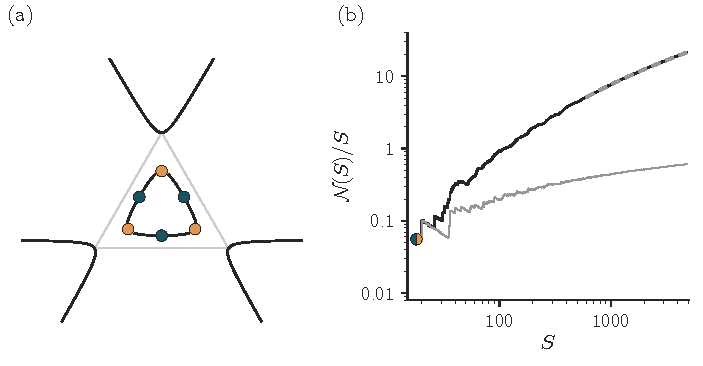
\includegraphics[width=119mm]{figures/out/F9.pdf}
\caption{(a) The real locus of $C_{27/2}$ in the chart $x+y+z=1$, with the permutations of $(1,4,4)$ and $(1,1,4)$, that is, $(2,8,8)$ and $(3,3,12)$ up to scale. (b) $\N(S)/S$ (heavy) and its fit (dashed), far above the isosceles lower bound of Theorem~\ref{thm:iso}, which grows like $(\ciso+o(1))\log S$ (thin).}\label{fig:F9}
\end{figure}

\subsection{What Conjecture~\ref{conj:intro} would require}\label{sec:heuristic}

By Theorem~\ref{thm:loglog} and Proposition~\ref{prop:upper}, the exponent of growth of $\N$ lies between $1$ and $3$. The data place the local exponent at $1.58$ near $X=6000$, still falling. That is consistent with $\N(X)=X^{1+o(1)}$, but it does not exclude a limiting exponent anywhere between $1$ and about $1.58$. Conjecture~\ref{conj:intro} is an extrapolation, and we state what it says about the geometry.

Parametric families are the natural source of many coincidences. Consider a family in which the entries of both triples are forms of degree $d$ in $m$ variables. It contributes about $X^{m/d}$ pairs with sum at most $X$, up to logarithms and local densities. Remark~\ref{rem:nolinear} rules out $d=1$ apart from scaling. The isosceles family has $d=2$ and $m=2$: it is a rational \emph{curve} in the space of pairs up to scaling, and it gives $X\log X$ once the copies are counted. The dual family of Corollary~\ref{cor:dual} is a rational surface given by cubic forms in three variables ($d=3$, $m=3$), and its conic-bundle part gives $X(\log X)^2$ (Theorem~\ref{thm:loglog}). A rational surface parametrized by quadratic forms in three variables ($d=2$, $m=3$) would give about $X^{3/2}$, more than the conjecture allows. Conjecture~\ref{conj:intro} therefore implies in particular that the variety of pairs contains no such surface with a positive real point. We have not searched for one. We searched for one-parameter families only: a line in $\PP^2$ of triples $(x:y:z)$ is a family linear in its parameter, and two lines (possibly equal) give a family of coincidences when $\Lambda$ agrees on them after a M\"obius change of parameter. Among the $189$ lines meeting the positive triangle with coefficients of absolute value at most $7$, the only such families are the conics of the dual family, one Vieta involution on each line through a vertex. Since $84\%$ of the primitive pairs up to $4800$ are not dual pairs, the data do not show which subvarieties carry most of the coincidences.

The variety in question has a classical description. The map $(P,P')\mapsto(e_1(P')P,\,e_1(P)P')$ identifies pairs of points on a common $C_\Lambda$ with pairs of triples with equal sum and equal reciprocal sum. So the variety of pairs is birational to the fibre square $\mathcal E\times_{\PP^1}\mathcal E$ of the rational elliptic surface $\mathcal E\to\PP^1_\Lambda$ obtained by blowing up the nine base points of the pencil. All singular fibres of $\mathcal E$ are of type $I_n$. Fibre products of this kind were studied by Schoen \cite{schoen1988}, who showed that suitable resolutions are Calabi--Yau threefolds \cite[Prop.~7.1]{schoen1988}. Conjecture~\ref{conj:intro} is a statement about the positive rational points of bounded height on this threefold. Our counts come from rational curves and surfaces inside it, and from positive-rank fibres over individual values of $\Lambda$.

\section*{Acknowledgements}
The colours of Figure~\ref{fig:F9} are from the Scientific Colour Maps \cite{crameri2023}, which are designed to be perceptually uniform and readable by people with colour-vision deficiencies \cite{crameri2020}.

\section*{Statements and declarations}

\subsection*{Funding}
No funding was received for this work.

\subsection*{Competing interests}
The authors have no competing interests to declare that are relevant to the content of this article.

\subsection*{Ethics approval and consent}
Not applicable.

\subsection*{Data and code availability}
All code and data are in the public repository \url{https://github.com/Ali-M658/Arithmetic-verification}. The enumeration, the fits and the rank computations are produced by scripts of the repository, which also holds their independent re-derivations, the extension to $S\le6000$ and the remaining checks of this note. An archived copy will be deposited at Zenodo: \textbf{[PLACEHOLDER: Zenodo DOI, to be minted at submission.]}

\subsection*{Author contributions}
\textbf{[PLACEHOLDER: author contribution statement, to be supplied by the authors before submission.]}

\subsection*{Use of AI tools}
\textbf{[PLACEHOLDER: statement on the use of AI tools in preparing this manuscript, to be written by the authors.]}

\bibliographystyle{amsplain}
\bibliography{references}

\end{document}
